\section{Realisation}
\label{sec:realisation} 
\begin{wrapfigure}[15]{r}{.60\textwidth}
\centering\vspace{-2\baselineskip}
  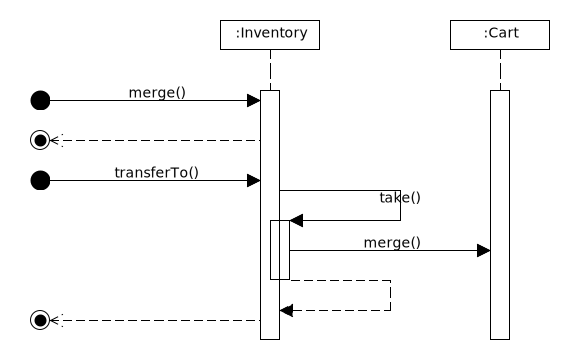
\includegraphics[width=.9\linewidth]{figures/fillInventorySellProduct_seqd}
  \caption{\label{seq:mergandtransfer}Fill the inventory (merge), then
    put a product from inventory into a cart.}
\end{wrapfigure}%
In figure~\ref{seq:mergandtransfer} you see a simplified model of the most
important business use case.
%
The application provides two implementations of the interface 
\Code{ProductContainer}:
\begin{enumerate*}
\item \Code{IMProductContainer} which is a hybrid file system / in memory implementation.
\item \Code{PGDBProductContainer} which uses a database (in particular
  postgresql) as the persistence service.
\end{enumerate*}

See the class diagram figure~\ref{fig:classdiagram} on
page~\pageref{fig:classdiagram} for details on class relations.

In this exam you will have to test and implement some of the methods.
The test names and documentation should give you hints on what to
test. After you have written the tests, you can implement the methods.

\subsection{The Façade between business and web}
In the design you find a Façade class, name \Code{WebshopFacade}, 
which provides one entry point to the whole business model. In the
class diagram you can find it too to see what methods are provided by
the \Code{webshopModel} project to the \Code{webshop} project.


\subsection{File system persistence}
The file system persistence implements a very simple approach, using one file
per (composite) object to persist. The only type that is currently persisted in
this way is the \Code{Invoice}. The files a stored in a sub directory,
simple named by type (Invoice in the example). The entity is stored in
a file named after its \textit{``primary key''}, with the file extension 
\texttt{.ser}. For instance, invoice with  number 31 is saved in file \texttt{fsdb/Invoice/31.ser}
%\clearpage
\subsection{RDMBS Persistence implementation}

\setlength{\intextsep}{0pt}
\begin{wrapfigure}[20]{r}{.35\linewidth}\vspace{-2\baselineskip}  
  \includegraphics[width=\linewidth]{figures/simpleschema.pdf}
  \caption{\label{fig:dbschema}Simplified database schema}
  \vspace{2\baselineskip}  
\end{wrapfigure}%

In the realisation of the persistence version 
(\Code{PGDBProductContainer}) of the product 
container, the responsibility of some of the constraints
(e.g. quantity of a product must be non-negative) can be delegated to
the database. When such a constraint is violated, the database layer
will throw an exception, which is wrapped into a \Code{java.lang.RunException} 
but should be caught, inspected (unwrapped with \Code{Exception.getCause()} 
and dealt with in a business appropriate way. 

The database schema can be found in figure~\ref{fig:dbschema}.

Note that the \Code{owner\_session} column identifies the cart, in case you
wonder why there is no \texttt{cart\_id} column in the \texttt{carts} table.



